\chapter{Related Works}


\section{Neural Networks}
    Neural networks are the most widely used method for many different applications including semantic segmentation. 
    Neural Networks are used to map a non-linear input to an output. 
    A neural network is made up of its input layer, any number of hidden layers and an output layer \cite{DeepLearning2015}.
    Neural networks are inspired after neurons in the brain \cite{DeepLearning2015}, \cite{Goodfellow-et-al-2016}, \cite{10.1371/journal.pcbi.Neurons}. 
    Each element within the vector of the input layer can be seen as a "neuron" where each element is interconnected and takes the information before it to make a decision and send it to another "neuron".
    This makes it so that as the layers go deeper in a neural network, the neurons are able to learn more and more complex things from the previous neurons.
    \par
    The input layer consists of the input for the task the network is supposed to learn. 
    For example for the image classification and segmentation tasks, usually the input would be the image the network is supposed to classify. 
    The hidden layers can be seen as a function that tries to predict the output. 
    Each hidden layer applies a function to the previous layer; each subsequent hidden layer is able to predict a more complex function.
    The output of the first and hidden layers is a feature map that the model will use in the subsequent layer \cite{Goodfellow-et-al-2016}. 
    The output layer finally consists of the probabilities associated with the final output 
    For example for image classification the output layer would be associated to a probability for each class, while for semantic segmentation, each pixel would have a probability associated with it for each class. 
    A basic neural network is shown in figure ~\ref{fig_neuralNetwork}. On the right we see the basic outline of the network with the input layer at the bottom with x, the hidden layer represented by h, and the output layer represented by y. Along each arrow is a W or a weight associated with the output of the previous layer. On the left shows a vectorized view of the right where each layer can have multiple elements.
    
    
\begin{figure}[tbh]
\centering
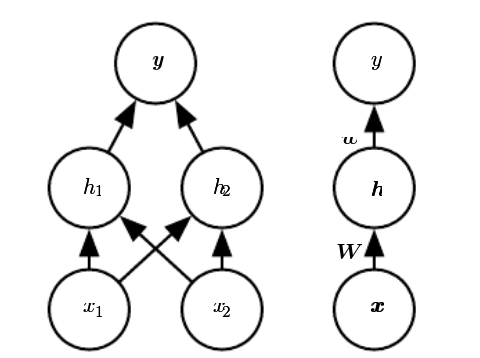
\includegraphics[width=\textwidth]{neural_network.png}
% where an .eps filename suffix will be assumed under latex,
% and a .pdf suffix will be assumed for pdflatex
\caption{This is an example of a neural network and its different representations on the left and right side. Image is from \cite{Goodfellow-et-al-2016}.}
\label{fig_neuralNetwork}
\end{figure}    


\subsection{Convolutional Neural Networks}
Convolutional Neural Networks or CNN's have had huge success with the task of semantic segmentation \cite{Girshick_2014_CVPR}, \cite{Long_2015}. 
Convolutional Neural Networks are one type of Neural Network, but a convolutional layer receives its input from multiple output nodes.
This allows convolutional neural networks to capture local information. 
The output of these convolutional layers is a feature map of the previous layer which takes a linear combination of the input to that layer \cite{Lee:2011:ULH:2001269.2001295}.
This allows for the model to learn complex shapes and use them to get the correct final output. 
The features that the convolutional neural network will learn depend on the task the network is trained for.
Figure ~\ref{fig:feature_map} shows the feature maps for a convolutional neural network trained on the segmentation of a region in an image. 
Figure ~\ref{fig:first_feature} show the output of 24 different filters of the first layer of a neural network trained on. Figure ~\ref{fig:second_feature} show the output of 100 different filters created from a linear combination of any number of filters in the first layer. 
This can be seen as in the first layer the feature maps are straight or curved lines usually, but for the second layer there are also circles or multiple different lines within the feature map.
The network learned straight or curved lines in the first layer or more complex shapes in the second layer as the network was trained to segment an image.
It is beneficial to increase the number of filters as we go deeper in the network so that the model can use more combinations of the previous layers features. 
There is no standard for the exact number of features one should use in a model as it depends on the task and how much the network would have to learn.

\begin{figure}
\centering
\begin{subfigure}{.5\textwidth}
  \centering
  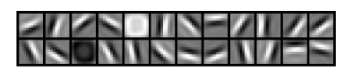
\includegraphics[width=.6\linewidth]{first_layer_features.png}
  \caption{}
  \label{fig:first_feature}
\end{subfigure}%
\begin{subfigure}{.5\textwidth}
  \centering
  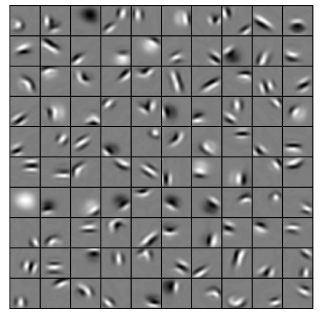
\includegraphics[width=.6\linewidth]{Second_layer_features.png}
  \caption{}
  \label{fig:second_feature}
\end{subfigure}
\caption{This network was trained on the segmentation of an image. The feature maps of the first (a) and second (b) layers are shown above. }
\label{fig:feature_map}
\end{figure}
    
\subsubsection{Convolution}
    Convolution is the element wise multiplication and addition of an image and a kernel. 
    Let $L:Z^2 \rightarrow R $ be a discrete function. 
    Let f be a discrete filter of size $(2r+1)^2 $. 
    The convolution operation $*$ can be shown as
\begin{equation}
 (L * f)(s) = \sum_{n+p=s}\sum_{m+p=s} L(m,n)f(p)\label{eq:convolution}
\end{equation}
    
    An example of this is shown in ~\ref{fig_convolutionOperation}. 
    The input is the image or feature map from a previous layer while the kernel matrix is the weight matrix learned by the model. 
    Each output pixel or feature map is calculated by the dot product of the kernel and appropriate image patch and then is moved across the image one pixel at a time. 
    This movement of the kernel across the image is called the stride and is usually 1 in order to not miss any important features that the model might see and get the best performance \cite{pmlr-v15-coates11a}. 
    Usually the kernel used is much smaller than the image in question in order to have sparse connections.
    This leads the model to learn small meaningful features as the output \cite{Goodfellow-et-al-2016}. 
    In convolution layers the kernel matrix is held constant so as to prevent over fitting and ease training. 

\begin{figure}[tbh]
\centering
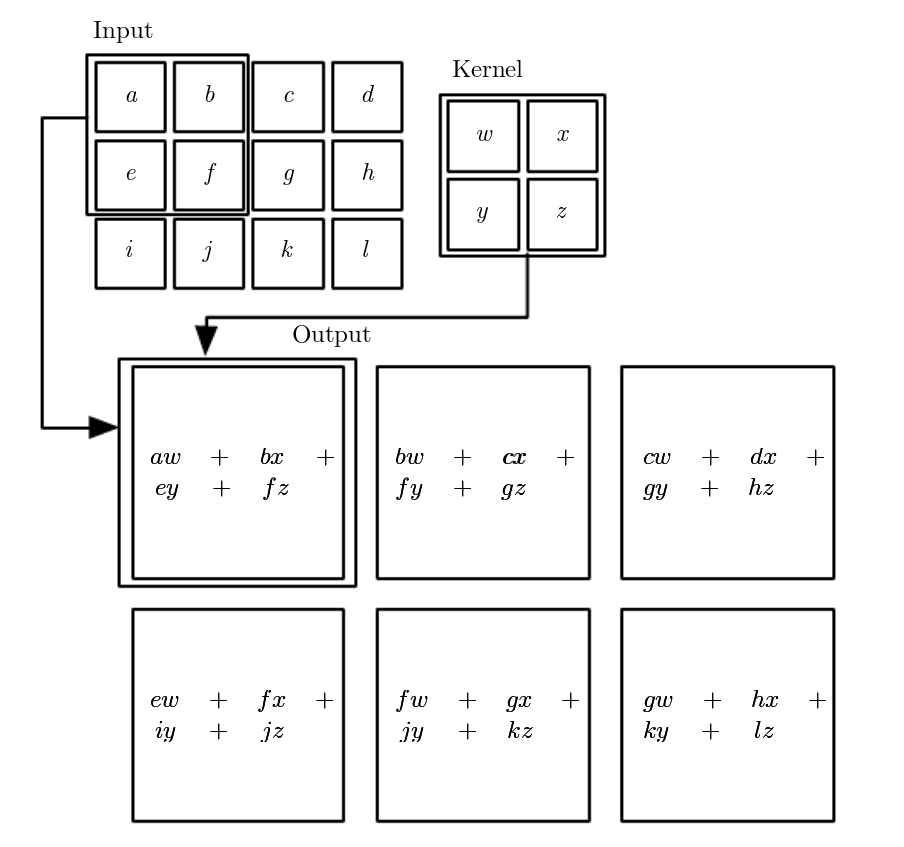
\includegraphics[width=\textwidth]{convolution_operation.png}
% where an .eps filename suffix will be assumed under latex,
% and a .pdf suffix will be assumed for pdflatex
\caption{This is an example of the convolution operation as it is applied to images. Image is from \cite{Goodfellow-et-al-2016}.}
\label{fig_convolutionOperation}
\end{figure} 


\subsubsection{Dilated Convolution}
    Dilated convolutions are different from regular convolutions because they apply the same convolutional filter at different receptive field sizes according to the dilation rate \cite{Yu2016MultiScaleCA}.
    The filter applied to the input has spaces in between the elements corresponding to the dilation rate.
    If we take the convolution operator definition and add $d$ be the dilation factor then the convolution operation can be shown as 
\begin{equation}
 (L *_d f)(s) = \sum_{m+dn=s} L(m)f(n)\label{eq:dilconvolution}
\end{equation}

     According to the dilation rate the filter is applied to different parts of the image, increasing the receptive field size \cite{DBLP:journals/corr/ChenPSA17}. 
     If we define $i$ to be the dilation factor then we can define the filters with increasing dilation as
    
\begin{equation}
 L_{i+1} = L_{i*2^i} f \qquad \mbox{for   } i = 0,1,...,n\label{eq:dilatedrate} 
\end{equation}
    
    An example of three different types of dilation are shown in figure ~\ref{fig_dil_convolution}. The first image on the left shows a dilation of 1 which corresponds to a dilation factor of 0 and is a normal kernel applied to the input which corresponds to a receptive field size of 3x3. The second image in the middle shows a dilation of 2 or dilation factor of 1 applied to the input and correspondingly a receptive field size of 7x7. The last image on the right shows a dilation of 4 or dilation factor of 2 applied to the input with a receptive field size of 15x15.
    As the dilation rate increases the receptive field size increases by $(2^{i+2}-1)$x$(2^{i+2}-1)$ where $i$ corresponds to the dilation factor.
    The dilation can be computed by $2^i$ where $i$ is the dilation factor ranging from 0 to n. 
    Dilated convolutions allow the receptive field size to increase exponentially without losing image resolution.
    Regular convolutional layers would need to go much deeper in order to get the receptive field size that dilated convolutions can have.
    
\begin{figure}[tbh]
\centering
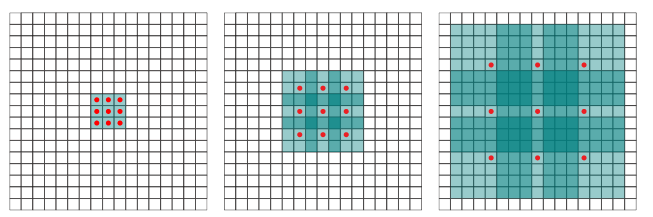
\includegraphics[width=\textwidth]{dilated_convolutions.png}
% where an .eps filename suffix will be assumed under latex,
% and a .pdf suffix will be assumed for pdflatex
\caption{This image shows the different types of dilation rates and how it affects the receptive field sizes of a 2D image. Image is from \cite{Yu2016MultiScaleCA}. }
\label{fig_dil_convolution}
\end{figure}     

\subsection{Activation Functions}    
    Neural networks not only need convolutional layers, but activation functions in order do a lot of the tasks we need.
    This is because without activation functions the model would just be a huge linear model, which while useful is not able to account for more complex cases.
    Activation functions help to add a non linearity to the neural network to help it learn more complex tasks.
    Many different types of activation functions have been used in the history of neural networks. 
    The standard was to use $f(x) = tanh(x)$  or sigmoid, $f(x) = 1/(1+e^{-x})$, as the output function for every layer. 
    It was later proved that ReLu or Rectified Linear Units actually trained convolutional neural networks several times faster \cite{NIPS2012_Krizhevsky}. ReLu also was proven to approximate all functions dimension n as long as the width of the network was greater than n \cite{NIPS2017_ReLuUniversalTheorem}. 
    ReLu is a nonlinear function defined as $f(x) = max(0, x)$. 
    This simple function allowed for faster training time because the tanh function saturates after a certain point as seen in figure ~\ref{fig:activation}. 
    This means that for values farther from zero the values will barely change. 
    This is fixed with ReLu as it never fully saturates which allows for easier training. 
    ReLu also preserves some of the linearity which allows for easier optimization and better generalization \cite{Goodfellow-et-al-2016}. 
    This thesis uses ReLu activation function for all the convolution layers.

\begin{figure}
\centering
\begin{subfigure}{.5\textwidth}
  \centering
  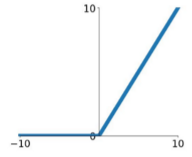
\includegraphics[width=.6\linewidth]{ReLu.png}
  \caption{plot of ReLu function $f(x) = max(0,x)$}
  \label{fig:ReLu}
\end{subfigure}%
\begin{subfigure}{.5\textwidth}
  \centering
  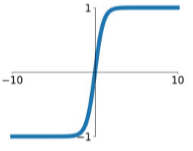
\includegraphics[width=.6\linewidth]{tanh(x).png}
  \caption{plot of tanh function $f(x) = tanh(x)$.}
  \label{fig:tanh}
\end{subfigure}
\caption{This figure shows some common activation functions.}
\label{fig:activation}
\end{figure}

\subsection{Pooling}
    Convolutional layers with non linear activation functions are not enough for models to learn well. 
    Whenever there are convolutional layers most of the time there are also layers that shrink the representation of the convolutional layers as it greatly helps the model train \cite{Lee:2011:ULH:2001269.2001295}. 
    Pooling just takes a small subsample of the input and combines it into one pixel output. 
    The size of the subsampled input is determined by the filter size of the pooling layer. 
    A 3x3 filter will take 3x3 inputs and output a 1x1. 
    The pooling function would then be applied to the entire output using a sliding window. 
    Pooling layers help the model learn spatial invariance as well as reduce the dimensionality of the feature map \cite{Scherer:2010:EPO:1886436.1886447}. 
    Average pooling was widely used in the start of invent of convolutional neural networks \cite{NIPS2012_Krizhevsky}. 
    Average pooling applies the average function to the subsample input and outputs the average of all the pixels. 
    This was used until it was shown that another function, max, was better for learning \cite{Scherer:2010:EPO:1886436.1886447}. 
    Max pooling is the same idea as average pooling just instead of taking the average the maximum value would be taken. 
    Max pooling preforms better because it preserves the most important or highly weighted features. 
    In comparison, average pooling takes into account the features which might not be as important for the task.
    When used in convolutional neural networks, it helps the model learn spatially invariant features as the convolution operation is also spatially invariant itself. 
    An example of max pooling is shown in figure ~\ref{fig_max_pool}. 
    The 4x4 input is being applied to a 2x2 max filter where the maximum value is taken from the filter. 

\begin{figure}[tbh]
\centering
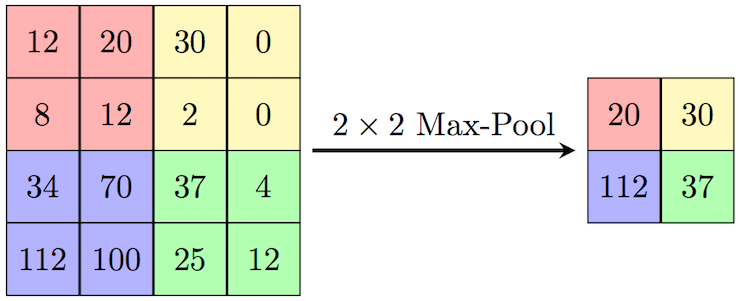
\includegraphics[width=0.75\textwidth]{max_pooling.png}
% where an .eps filename suffix will be0 assumed under latex,
% and a .pdf suffix will be assumed for pdflatex
\caption{ This is an example of max pooling on a 4x4 input with filter size 2x2.   }
\label{fig_max_pool}
\end{figure} 

\subsection{Batch Normalization}
    Convolutional neural networks are difficult to train. 
    The fact that the weights of every layer change every iteration as the deep network learns makes it so that even a small change in the beginning of the network will get amplified as it goes deeper in the network.
    This problem is the internal covariate shift in the network and can be fixed using batch normalization. 
    Batch normalization normalizes each layer in the network for each training batch. 
    Batch normalization is shown in figure ~\ref{fig_batch_norm}. 
    The input would be a minibatch and the output would be the input normalized using the mini-batch mean and variance while also scaled and shifted. 
    The batch normalization layers also add parameters for the network to learn, scale and shift.
    Batch normalization is used to help reduce the problem of the vanishing or exploding gradient and allow for the use of higher learning rates \cite{DBLP:journals/corr/IoffeS15}. 
    This will help models become more stable as well as train faster. 
    The use of batch normalization also helps to regularize the model and prevent overfitting \cite{DBLP:journals/corr/IoffeS15}. 
    Since batch normalization utilizes mini-batches then it will be less useful for batch sizes that are small as the variance in the batches will be greater.

\begin{figure}[tbh]
\centering
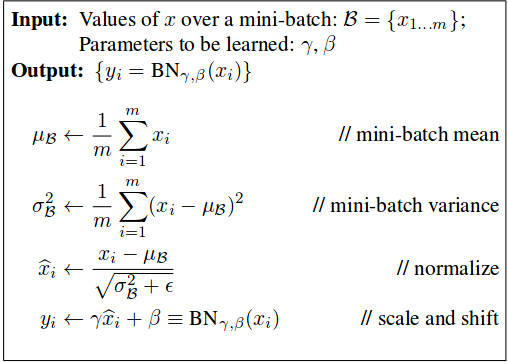
\includegraphics[width=0.5\textwidth]{batch_norm.png}
% where an .eps filename suffix will be0 assumed under latex,
% and a .pdf suffix will be assumed for pdflatex
\caption{ This is how batch normalization would be implemented in the model. Image is from \cite{DBLP:journals/corr/IoffeS15}. }
\label{fig_batch_norm}
\end{figure} 





